\documentclass[11pt,reqno]{amsart}

\usepackage{amsmath,amssymb,amsthm,amsfonts,mathtools}
\usepackage{tikz}
\usepackage[hidelinks]{hyperref}
\usepackage[a4paper,margin=1in]{geometry}
\usepackage{caption}
\captionsetup[table]{position=below,skip=12pt}

% Tolerate long, unbreakable \texttt{...} Lean identifiers without
% producing visible right-margin overruns.
\tolerance=2000
\emergencystretch=5em
\hbadness=2000   % don't warn about minor underfull \hbox
\hyphenpenalty=50

\theoremstyle{plain}
\newtheorem{theorem}{Theorem}[section]
\newtheorem{lemma}[theorem]{Lemma}
\newtheorem{corollary}[theorem]{Corollary}
\newtheorem{proposition}[theorem]{Proposition}

\theoremstyle{definition}
\newtheorem{definition}[theorem]{Definition}

\theoremstyle{remark}
\newtheorem{remark}[theorem]{Remark}
\newtheorem{example}[theorem]{Example}

% Shorthands
\newcommand{\Z}{\mathbb{Z}}
\newcommand{\R}{\mathbb{R}}
\newcommand{\N}{\mathbb{N}}
\newcommand{\Q}{\mathbb{Q}}
\newcommand{\fract}[1]{\{#1\}}
\newcommand{\etap}{\eta^{+}}
\newcommand{\etam}{\eta^{-}}
\newcommand{\mpl}{m^{+}}
\newcommand{\mmi}{m^{-}}
\newcommand{\orb}{\mathcal{O}}
\newcommand{\code}[1]{\texttt{#1}}

\title[A Lean 4 Formalization of the Three-Gap Theorem]{%
  A Lean~4 Formalization of the Three-Gap (Steinhaus) Theorem,
  Uniform in the Rotation Number}

\author{Dirk Kunert}
\address{Independent Researcher}
\email{dirk.kunert@gmail.com}

\subjclass[2020]{Primary 11K06, 68V20; Secondary 11J71, 11B57, 37B10, 52C05}
\keywords{three-gap theorem, Steinhaus conjecture, three-distance theorem,
Lean~4 formalization, machine-checked proof, interactive theorem proving,
Mathlib, first-return map, fractional parts, gap sequences, rotation}

\date{June 22, 2026}

\begin{document}

\begin{abstract}
We present a Lean~4 / Mathlib formalization of the three-gap (Steinhaus)
theorem: for every real number~$a$ and every $N\in\N$, the point set
$\{ia \bmod 1 : 0 \le i < N\}$ partitions the half-open interval $[0,1)$ into
gaps taking at most three distinct lengths, and when there are exactly three
the largest is the sum of the other two.  The formalization follows the
first-return (Slater--van Ravenstein) route, working throughout in $[0,1)$
via \code{Int.fract} rather than \code{AddCircle}.  To our knowledge this is
the first formalization of the theorem in Lean~4, and the first in any system
to treat rational and irrational~$a$ uniformly: the only previous formal
proof---Mayero's Coq development after van Ravenstein---is restricted to
irrational~$a$.  The geometric crux, that the longest gap contains no orbit
point, is discharged in the corner case by a self-contained
return-time/period argument: were a point to sit inside the gap, the two
indices realizing it would differ by a period strictly greater than the
positive return time and strictly less than the sum of the two return times,
contradicting their minimality.  This removes the irrationality
hypothesis of the van Ravenstein--Mayero line.  Both the distinct-count bound
\code{three\_gap\_card\_le\_three} and the sum relation
\code{three\_gap\_lengths\_eq} are proved with no \code{sorry}, depending only on
the axioms \code{propext}, \code{Classical.choice}, \code{Quot.sound}; the
development is about $1{,}480$ lines.  We do \emph{not} claim a new proof
of the theorem: elementary proofs valid for all~$a$ are classical---for
instance Liang's $1979$ rigid-gap argument---and our contribution is the
machine-checked formalization together with the formalization-friendly corner
argument that makes the first-return route uniform.
\end{abstract}

\maketitle

% =====================================================================
\section{Introduction}\label{sec:intro}
% =====================================================================

Fix a real number~$a$ and a positive integer~$N$, and place the $N$ points
\[
  \fract{0\cdot a},\ \fract{1\cdot a},\ \dots,\ \fract{(N-1)a}
\]
on the circle $\R/\Z$, identified throughout with the half-open interval
$[0,1)$ via the fractional part $\fract{x} = x - \lfloor x\rfloor$.  These
points cut the circle into arcs.  The \emph{three-gap theorem}---conjectured by
Hugo Steinhaus and first proved in the late $1950$s by
S\'os~\cite{Sos1958}, Sur\'anyi~\cite{Suranyi1958}, and
\'Swierczkowski~\cite{Swierczkowski1959}---asserts that these arcs take at most
three distinct lengths, and that whenever there are exactly three, the longest
is the sum of the other two.  The result, also known as the three-distance
theorem, has since accumulated many proofs and a large literature
(see~\cite{BertheReutenauer2024} for a recent survey); we recall the proof
landscape in Section~\ref{sec:related}.

The present paper concerns not a new proof but a \emph{machine-checked} one.
We describe a formalization of the three-gap theorem in the Lean~4 interactive
theorem prover~\cite{Moura2021} on top of its mathematical library
Mathlib~\cite{Mathlib2020}.  The central statement, in the notation developed
below, is the following.

\begin{theorem}[\code{three\_gap\_card\_le\_three}]\label{thm:main}
For every $a\in\R$ and every $N\in\N$, the multiset of gaps of the points
$\{ia \bmod 1 : 0 \le i < N\}$ takes at most three distinct values.
\end{theorem}

Theorem~\ref{thm:main} is proved in Lean with no \code{sorry}, and a kernel
check reports that it depends only on the three foundational axioms
\code{propext}, \code{Classical.choice}, and \code{Quot.sound} that underlie
Mathlib itself---nothing specific to this development is assumed.  The complete
source is a single self-contained module of roughly $1{,}480$ lines.

\subsection*{The first-return route}
Our formalization follows the \emph{first-return} viewpoint of
Slater~\cite{Slater1967} and van Ravenstein~\cite{vanRavenstein1988}.  Two
distinguished orbit points govern the gap structure: the smallest positive
point $\etap$ (the \emph{positive return}) and $\etam = 1 - \max$, the gap from
the largest point up to~$1$ (the \emph{negative return}).  Each point's
right neighbour is obtained either by adding the index of~$\etap$ or by
subtracting the index of~$\etam$, according to a purely arithmetic condition on
indices; this yields gaps of length $\etap$ or $\etam$ directly.  The whole
difficulty is concentrated in the \emph{corner} case, where both index
conditions fail: here the gap equals $\etap+\etam$, and one must show that the
long gap of length $\etap+\etam$ is \emph{empty}, i.e.\ contains no orbit point
in its interior.  This emptiness is the geometric heart of the theorem.

\subsection*{Uniformity and prior formalization}
A noteworthy feature of the formalization is that it is \emph{uniform in~$a$}:
the same proof covers rational and irrational rotation numbers, with no case
split.  This is not automatic for the first-return route.  Van Ravenstein's
proof, and the only previous formalization of the theorem---Mayero's Coq
development~\cite{Mayero2000}, which follows van Ravenstein---assume $a$
irrational, so that distinct indices always give distinct points; the rational
case, where the orbit is periodic and indices collide, is set aside.  We close
the corner case for all~$a$ at once.  The collision of two indices on the same
orbit point is exactly a \emph{period} of the rotation, and we show that in the
corner such a period would lie strictly between the positive return index and
the sum of the two return indices, contradicting their minimality.  For irrational~$a$ no nonzero period exists and
the argument specializes to the classical situation; for rational~$a$ it
supplies precisely the step that the van Ravenstein--Mayero line omits.

\subsection*{What we do and do not claim}
We make a deliberately narrow claim.  To our knowledge this is the first
formalization of the three-gap theorem in Lean~4---the theorem is absent from
Mathlib at the time of writing---and the first machine-checked proof, in any
system, valid uniformly for rational and irrational~$a$.  We do \emph{not}
claim a new proof of the theorem itself.  Elementary proofs valid for
all~$a$ have long been available: Liang's $1979$ ``rigid gap''
argument~\cite{Liang1979}, for instance, is uniform and self-contained.  We
survey the proof landscape, including the dynamical and geometric proofs, in
Section~\ref{sec:related}.  The minimality of the two return times is, moreover,
the engine of every proof in the first-return family.  Our contribution is the
formalization, and the particular packaging of the corner step---through a
period/minimality contradiction---that makes the first-return route uniform and
convenient to verify mechanically.

\subsection*{Outline}
Section~\ref{sec:setup} sets up the orbit, the gap multiset, and the two
returns, and records the reduction of Theorem~\ref{thm:main} to a
three-element containment.  Section~\ref{sec:cases} treats the two
straightforward cases~A ($\etap$) and~B ($\etam$).
Section~\ref{sec:corner} is the heart: the corner case, the auxiliary
``$M$-circle'' on which the empty-gap lemmas are proved, and the
period/minimality argument that closes the last step; it ends with a fully
worked rational example.  Section~\ref{sec:lean} describes the Lean
development---its architecture, design choices, a correspondence table between
the paper and the formal text, and the scope of trust.
Section~\ref{sec:related} surveys the known proofs and locates ours among
them, and Section~\ref{sec:discussion} discusses a possible Mathlib
contribution and further directions.

% =====================================================================
\section{Orbit, Gaps, and the Two First Returns}\label{sec:setup}
% =====================================================================

Throughout, $a\in\R$ and $N\in\N$ are fixed, and $\fract{x}=x-\lfloor x\rfloor
\in[0,1)$ denotes the fractional part.  We work in $[0,1)$ via \code{Int.fract}
rather than in the quotient \code{AddCircle}; this keeps every quantity an
honest real number and lets all order- and difference-arguments run directly in
$\R$.  Because equality and order on $\R$ are noncomputable in Lean, every
object below is declared \code{noncomputable}, which is immaterial for proving.

\subsection{The orbit and its enumeration}

\begin{definition}[\code{orbit}, \code{orbitCard}]
The \emph{orbit} is the finite set of distinct points
\[
  \orb(a,N) \;=\; \bigl\{\, \fract{i\,a} \;:\; 0 \le i < N \,\bigr\}
  \;\subseteq\; [0,1),
\]
realized in Lean as \code{(Finset.range N).image (fun i => Int.fract (i*a))}.
Its cardinality is \code{orbitCard a N}, written~$k$ below.  As $\fract{0\cdot
a}=0$, the point $0$ lies in every nonempty orbit.
\end{definition}

The points of $\orb(a,N)$, listed in increasing order, are denoted
$x_0 < x_1 < \dots < x_{k-1}$.  In Lean this enumeration is
\code{sortedVal a N}, a total function $\N\to\R$ defined from Mathlib's
order isomorphism \code{Finset.orderEmbOfFin} on the first $k$ indices (and set
to a junk value $0$ beyond, which never matters).  We write
$x_i = \code{sortedVal a N i}$.  It is strictly increasing on $0,\dots,k-1$
(\code{sortedVal\_strictMono}), with $x_0 = 0$
(\code{sortedVal\_zero\_eq\_zero}) and $x_{k-1} = \max\orb(a,N)$
(\code{sortedVal\_last}).

\subsection{Gaps}

\begin{definition}[\code{gaps}, \code{gapAt}]
The \emph{gap multiset} of $\orb(a,N)$ is
\[
  \mathrm{gaps}(a,N) \;=\;
  \bigl\{\, x_{i+1}-x_i \;:\; 0 \le i < k-1 \,\bigr\}
  \;\uplus\;
  \bigl\{\, x_0 + 1 - x_{k-1} \,\bigr\},
\]
the $k-1$ consecutive differences together with the single \emph{wrap-around}
gap from the largest point up across $1$ to the smallest.  The $i$-th internal
gap is $\code{gapAt a N i} = x_{i+1}-x_i$.
\end{definition}

\begin{lemma}[\code{gaps\_sum\_eq\_one}]\label{lem:sum-one}
If $N>0$ then the entries of $\mathrm{gaps}(a,N)$ sum to~$1$.
\end{lemma}

\begin{proof}[Proof idea]
The consecutive differences telescope to $x_{k-1}-x_0$; adding the wrap-around
gap $x_0+1-x_{k-1}$ gives~$1$.  In Lean this is \code{Finset.sum\_range\_sub}
followed by \code{ring}.
\end{proof}

Membership in the gap multiset unpacks (\code{mem\_gaps\_iff}) into ``$y$ is an
internal gap $\code{gapAt a N i}$ for some $i<k-1$, or $y$ is the wrap-around
gap''.

\subsection{The two first returns}

\begin{definition}[\code{etaPos}, \code{etaNeg}]\label{def:returns}
Assume the orbit is nondegenerate, $k\ge 2$.  The \emph{positive return} is the
smallest positive orbit point,
\[
  \etap \;=\; \code{etaPos a N} \;=\; \min\bigl(\orb(a,N)\setminus\{0\}\bigr),
\]
and the \emph{negative return} is the complement of the largest orbit point,
\[
  \etam \;=\; \code{etaNeg a N} \;=\; 1 - \max\orb(a,N).
\]
\end{definition}

Both are positive: $\etap>0$ by construction, and $\etam>0$ because the maximum
of $\orb(a,N)\subseteq[0,1)$ is $<1$.  In Lean the positive points form
\code{posOrbit a N = (orbit a N).erase 0}, and $\etap,\etam$ are \code{min'} and
$1-\code{max'}$ of it.  The two returns are characterized by minimality:

\begin{lemma}[\code{no\_orbit\_below\_etaPos}, \code{le\_one\_sub\_etaNeg}]
\label{lem:return-min}
For every $y\in\orb(a,N)$ with $y>0$,
\[
  \etap \;\le\; y \;\le\; 1-\etam .
\]
That is, no orbit point lies in $(0,\etap)$ or in $(1-\etam,1)$.
\end{lemma}

Geometrically, $\etap$ is the length of the gap to the right of $0$
(\code{gapAt a N 0} $=\etap$, \code{gapAt\_zero\_eq\_etaPos}), and $\etam$ is the
wrap-around gap (\code{wraparound\_eq\_etaNeg}); so both returns already occur as
gap lengths.

\subsection{Reduction of the main theorem}

The number of \emph{distinct} gap lengths is the cardinality of the underlying
set $\mathrm{gaps}(a,N).\code{toFinset}$.  The entire proof is organized around
a single reduction.

\begin{lemma}[\code{three\_gap\_card\_le\_three\_of\_subset}]\label{lem:reduction}
If there exist reals $x,y,z$ with
$\mathrm{gaps}(a,N).\code{toFinset} \subseteq \{x,y,z\}$, then
$\mathrm{gaps}(a,N).\code{toFinset}$ has at most three elements.
\end{lemma}

Thus Theorem~\ref{thm:main} reduces to showing that \emph{every} gap value lies
in the three-element set $\{\etap,\,\etam,\,\etap+\etam\}$.  The degenerate
orbits are immediate: if $k\le 1$ there is a single gap
(\code{gaps\_card\_eq\_one\_of\_degenerate}), so from now on we assume $k\ge 2$.
The wrap-around gap equals $\etam$ (\code{wraparound\_eq\_etaNeg}, since
$x_0=0$ and $x_{k-1}=\max$), and \code{gapAt a N 0}
equals~$\etap$; the work is to classify every \emph{internal} gap
$\code{gapAt a N i}$ with $0<i$, which is the subject of the next two sections.

% =====================================================================
\section{The First-Return Classification: Cases A and B}\label{sec:cases}
% =====================================================================

To classify the internal gap to the right of an orbit point we recover the
\emph{index} behind each point and track how adding the two return indices moves
points around the circle.

\subsection{Canonical multipliers and return indices}

\begin{definition}[\code{canMul}, \code{mPlus}, \code{mMinus}]
For $p\in\orb(a,N)$, the \emph{canonical multiplier} $\code{canMul a N p}$ is the
least index $k<N$ with $\fract{k\,a}=p$ (the minimum of the nonempty
\emph{fibre} $\{k<N : \fract{k a}=p\}$).  The \emph{return indices} are the
canonical multipliers of the two returns:
\[
  \mpl = \code{mPlus a N} = \code{canMul a N}\,\etap,
  \qquad
  \mmi = \code{mMinus a N} = \code{canMul a N}\,(1-\etam).
\]
\end{definition}

Thus $\fract{\mpl a}=\etap$ and $\fract{\mmi a}=1-\etam=\max\orb(a,N)$, with
$0<\mpl<N$ and $\mmi<N$ (\code{mPlus\_lt}, \code{mMinus\_lt},
\code{mPlus\_pos}).  Adding a return index rotates a point by the corresponding
return, as recorded by the fractional-part identity $\fract{\fract{x}+\fract{y}}
=\fract{x+y}$ (\code{fract\_add\_fract\_eq}):

\begin{lemma}[\code{fract\_index\_shift}, \code{fract\_index\_shift\_noWrap}]
\label{lem:shift}
For every $j\in\N$, $\ \fract{(j+\mpl)\,a} = \fract{\fract{j a}+\etap}$.  In
particular, if $\fract{j a}+\etap<1$ (no wrap), then
$\fract{(j+\mpl)\,a}=\fract{j a}+\etap$.  The analogue with $\mmi$ rotates by
$1-\etam$, i.e.\ downward by $\etam$ (\code{fract\_index\_shift\_neg}).
\end{lemma}

\subsection{The two ``no point between'' lemmas}

The sorted enumeration leaves no orbit point strictly between consecutive
values: there is no $z\in\orb(a,N)$ with $x_i<z<x_{i+1}$
(\code{no\_orbit\_strictly\_between}).  The substance of cases A and B is that
adding a return index to an \emph{in-range} index produces no nearer point.

\begin{lemma}[\code{noPointBetween}]\label{lem:npb}
Let $j$ be an index with $j+\mpl<N$.  Then no orbit point lies in the open
interval $(\fract{j a},\,\fract{j a}+\etap)$.
\end{lemma}

\begin{proof}[Proof idea]
Suppose $z=\fract{w a}$ lies there, and set $d=z-\fract{j a}\in(0,\etap)$.  If
$w\ge j$, then $\fract{(w-j)a}=d$ is a positive orbit value below~$\etap$,
contradicting Lemma~\ref{lem:return-min}.  If $w<j$, the complementary index
$j-w$ realizes a point in the top band $(1-\etap,1)$; but $(j-w)+\mpl<N$ forces
$\fract{(j-w)a}+\etap\le 1$ (lemma \code{fract\_add\_etaPos\_le\_one}, the
in-range half of the argument), and the two facts are incompatible.  The
hypothesis $j+\mpl<N$ is exactly what keeps the shifted indices in range so that
minimality applies.
\end{proof}

The backward mirror \code{noPointBetween\_neg} states, symmetrically, that if
$j+\mmi<N$ then no orbit point lies in $(\fract{j a}-\etam,\,\fract{j a})$.

\subsection{Cases A and B}

Write $v=x_i$ and $v'=x_{i+1}$ for a consecutive pair, and let
$j=\code{canMul a N}\,v$ be the canonical index of the left point.

\begin{proposition}[Case A, \code{gap\_eq\_etaPos}]\label{prop:caseA}
If $j+\mpl<N$ then $\code{gapAt a N i}=\etap$.
\end{proposition}

\begin{proof}[Proof idea]
By Lemma~\ref{lem:shift} (no wrap, using \code{fract\_add\_etaPos\_le\_one}) the
point $v+\etap=\fract{(j+\mpl)a}$ is an orbit point, and $v<v+\etap<1$.  By
Lemma~\ref{lem:npb} nothing lies in $(v,v+\etap)$, and by
\code{no\_orbit\_strictly\_between} nothing lies in $(v,v')$; since $v+\etap$ is
an orbit point above $v$, the two facts force $v'=v+\etap$.
\end{proof}

\begin{proposition}[Case B, \code{gap\_eq\_etaNeg}]\label{prop:caseB}
Let $j'=\code{canMul a N}\,v'$ be the canonical index of the \emph{right} point.
If $j'+\mmi<N$ then $\code{gapAt a N i}=\etam$.
\end{proposition}

Proposition~\ref{prop:caseB} is the exact mirror of~\ref{prop:caseA}, obtained
by rotating $v'$ downward by $\etam$ and applying \code{noPointBetween\_neg}.
The two index conditions $j+\mpl<N$ and $j'+\mmi<N$ are the arithmetic
discriminant of the whole classification.  When at least one holds, the gap is
$\etap$ or $\etam$.  The remaining possibility---both fail---is the corner case
of the next section.

% =====================================================================
\section{The Corner Case}\label{sec:corner}
% =====================================================================

Keep the notation $v=x_i$, $v'=x_{i+1}$, $j=\code{canMul a N}\,v$, and
$j'=\code{canMul a N}\,v'$.  The \emph{corner} is the case in which both index
conditions of Section~\ref{sec:cases} fail:
\[
  j+\mpl \ge N \qquad\text{and}\qquad j'+\mmi \ge N. \tag{corner}
\]
The goal of this section is the following, after which Theorem~\ref{thm:main}
follows.

\begin{proposition}[\code{corner\_gap}]\label{prop:corner}
In the corner case, $\code{gapAt a N i}=\etap+\etam$.
\end{proposition}

Equivalently, $v'=v+\etap+\etam$: the long gap from $v$ skips over the missing
midpoint $v+\etap$ and lands on $v'$.  The proof has a prior \emph{discriminant}
step and the genuinely hard \emph{empty-gap lower bound}; the matching upper
bound is then a short closing step that depends on the lower bound, not an
independent ingredient.

\subsection{The discriminant \texorpdfstring{$j<\mmi$}{j < m-}}

\begin{lemma}[\code{corner\_canMul\_lt\_mMinus}]\label{lem:hP1}
In the corner case, $j<\mmi$.
\end{lemma}

\begin{proof}[Proof idea]
Suppose $j\ge\mmi$.  Then $\fract{(j-\mmi)a}=v+\etam$ is an orbit point at the
in-range index $j-\mmi<N$, lying above $v$.  One checks, using
Proposition~\ref{prop:caseB} for the point $v+\etam$, that its predecessor is
exactly $v$, so $v+\etam=v'$ and $\code{canMul a N}\,v'\le j-\mmi$.  Then
$j'+\mmi\le j<N$, contradicting the corner condition $j'+\mmi\ge N$.
\end{proof}

Lemma~\ref{lem:hP1} gives the bound we need for the next step: since $j<\mmi$,
\[
  j+\mpl \;<\; \mmi+\mpl \;=\; M ,
\]
so the forward shift of $v$ by $\mpl$ stays in range in the enlarged circle
$\orb(a,M)$ introduced below.  Write $q:=v+\etap+\etam$.  The whole task now is
the \emph{lower bound}: no orbit point lies in the open interval $(v,q)$.

Granting it, the corner proposition follows quickly.  The lower bound gives
$v'\ge q$, since $v'$ is the least orbit point above $v$; hence
$v+\etap+\etam=v'<1$, so $q<1$.  Only now is $q$ realized without wrap:
$q=\fract{(j+\mpl-\mmi)a}$, with index $j+\mpl-\mmi<N$ because $j<\mmi$ and
$\mpl<N$ give $j+\mpl<\mmi+N$.  Thus $q\in\orb(a,N)$, and as $q>v$ with nothing
strictly between $v$ and $v'$ we get the \emph{upper bound} $v'\le q$.  Together,
$v'=q=v+\etap+\etam$.  (Note the order: the upper bound uses $q<1$, which comes
from the lower bound---in the Lean proof the no-wrap realization of $q$ is
derived from \code{hLower}, not before it.)

\subsection{The \texorpdfstring{$M$}{M}-circle}

The obstacle is that in the corner the in-range ``no point between'' lemmas of
Section~\ref{sec:cases} do not apply at $v$: every index of $v$ has its forward
shift out of range.  We sidestep this by enlarging the orbit.  Put
\[
  M \;=\; \mpl+\mmi .
\]
By Lemma~\ref{lem:hP1} and the corner condition, $N\le j+\mpl<M$, so $N<M$ and
$\orb(a,N)\subseteq\orb(a,M)$ (\code{orbit\_mono}).  Crucially, the two returns
are \emph{unchanged} on passing to the larger circle.

\begin{lemma}[\code{etaPos\_eq\_extend}, \code{etaNeg\_eq\_extend}]
\label{lem:returns-preserved}
$\code{etaPos a M}=\etap$ and $\code{etaNeg a M}=\etam$.
\end{lemma}

\begin{proof}[Proof idea]
No new index $k\in[N,M)$ can produce a point in $(0,\etap)$ or in
$(1-\etam,1)$: such a $k$ would, after subtracting $\mmi$ resp.\ $\mpl$, yield a
point forcing $\mpl\le k-\mmi$ or $\mmi\le k-\mpl$, i.e.\ $k\ge\mpl+\mmi=M$,
contrary to $k<M$ (\code{no\_new\_below\_etaPos}, \code{no\_new\_above\_etaNeg}).
Hence the minimum positive point and the maximum are the same in $\orb(a,M)$ as
in $\orb(a,N)$.
\end{proof}

Because $j+\mpl<M$, the forward ``no point between'' lemma now \emph{does} apply
in $\orb(a,M)$, and dually for the backward one at $q$.  This yields the two
empty-interval halves, stated for the original orbit since
$\orb(a,N)\subseteq\orb(a,M)$.

\begin{lemma}[\code{corner\_noPoint\_lo}, \code{corner\_noPoint\_hi}]
\label{lem:L1L3}
In the corner case, no orbit point of $\orb(a,N)$ lies in $(v,\,v+\etap)$
(call this L1) or in $(v+\etap,\,q)$ (call this L3).
\end{lemma}

After L1 and L3, the only way the lower bound could fail is if the midpoint
$v+\etap$ itself were an orbit point.  Ruling this out is the last and deepest
step.

\subsection{The empty midpoint, without induction}

\begin{theorem}[L2, \code{corner\_gap} lower bound]\label{thm:L2}
In the corner case, $v+\etap\notin\orb(a,N)$.
\end{theorem}

\begin{proof}
Suppose $v+\etap=\fract{k\,a}$ with $k<N$.  Recall
$v+\etap=\fract{(j+\mpl)a}$, with $j+\mpl\ge N$ by the corner condition.

\emph{Case $k\ge j$.}  Then $\fract{(k-j)a}=\fract{k a}-\fract{j a}=\etap$ is an
orbit point realizing $\etap$ at index $k-j<N$, so by minimality of $\mpl$ we
have $\mpl\le k-j$, i.e.\ $k\ge j+\mpl\ge N$---contradicting $k<N$.  (This is
exactly where the corner condition $j+\mpl\ge N$ is used.)

\emph{Case $k<j$.}  Now $\fract{k a}=v+\etap=\fract{(j+\mpl)a}$ with
$k\ne j+\mpl$, so their difference is an integer multiple of~$a$ with vanishing
fractional part:
\[
  d := j+\mpl-k, \qquad \fract{d\,a}=0, \qquad \mpl<d<\mpl+\mmi .
\]
(The bounds are $d>\mpl$ from $k<j$, and $d\le j+\mpl<\mpl+\mmi$ from
Lemma~\ref{lem:hP1}.)  Thus $d$ is a \emph{period} of the rotation lying
strictly between $\mpl$ and $\mpl+\mmi$.  We derive a contradiction from the
minimality of $\mmi$ or of $\mpl$.

Since $d>\mpl$, the index $d-\mpl\in(0,\mmi)$ has
$\fract{(d-\mpl)a}=\fract{-\etap}=1-\etap$, an orbit point in the top band; by
Lemma~\ref{lem:return-min}, $1-\etap\le 1-\etam$, hence $\etam\le\etap$.  Now
compare $d$ with $\mmi$ (note $d\ne\mmi$, as $\fract{\mmi a}=1-\etam\ne0$):
\begin{itemize}
\item If $d<\mmi$, then $\fract{(\mmi-d)a}=\fract{(1-\etam)-0}=1-\etam$ realizes
the maximum at index $\mmi-d<\mmi$.  But $\mmi=\code{canMul a N}\,(1-\etam)$ is
the \emph{least} such index, a contradiction.
\item If $d>\mmi$, then $\fract{(d-\mmi)a}=\fract{-(1-\etam)}=\etam$ realizes
$\etam$ at index $d-\mmi<\mpl$.  Together with $\etam\le\etap$ and minimality of
$\etap$ (Lemma~\ref{lem:return-min}, which gives $\etap\le\etam$) we get
$\etap=\etam$; so $\etap$ itself occurs at index $d-\mmi<\mpl=\code{canMul a
N}\,\etap$, again contradicting minimality.
\end{itemize}
Either way the case $k<j$ is impossible, and $v+\etap\notin\orb(a,N)$.
\end{proof}

\begin{remark}[Why this is uniform in $a$]\label{rmk:uniform}
For irrational $a$ no nonzero period exists: $\fract{d a}=0$ with $d\ge1$ would
force $a=(\text{integer})/d\in\Q$.  So the case $k<j$ is vacuous, and L2 reduces
to the elementary case~$k\ge j$---this is the situation treated by van
Ravenstein and formalized by Mayero.  For rational $a$ the period is genuine,
and the bound $\mpl<d<\mpl+\mmi$ is precisely what rules it out: the minimal
period of the orbit is at least $\mpl+\mmi$ in the corner, so no period can sit in
that window.  The single argument above covers both regimes, which is what lets
the Lean proof avoid any rational/irrational case split.
\end{remark}

Combining L1, L3, and Theorem~\ref{thm:L2}: any orbit point in $(v,q)$ would lie
in $(v,v+\etap)$, equal $v+\etap$, or lie in $(v+\etap,q)$, all impossible.
Hence $v'\ge q$, which with the upper bound gives $v'=q=v+\etap+\etam$ and proves
Proposition~\ref{prop:corner}.

\subsection{Assembling the theorem}

Propositions~\ref{prop:caseA}, \ref{prop:caseB}, and~\ref{prop:corner} together
classify every internal gap: \code{neighbour\_gap\_in\_returns} states that
$\code{gapAt a N i}\in\{\etap,\etam,\etap+\etam\}$ for all $i$ with $i+1<k$.
(For $i=0$ no separate base case is needed: there $\code{canMul a N}\,v=0$ and
$\mpl<N$, so case~A fires.)  Adding the wrap-around gap, which equals $\etam$,
\code{gaps\_subset\_returns} gives
\[
  \mathrm{gaps}(a,N).\code{toFinset}\ \subseteq\ \{\etap,\,\etam,\,\etap+\etam\},
\]
and Lemma~\ref{lem:reduction} yields Theorem~\ref{thm:main}.  The classical
\emph{sum relation} is the immediate complement: since the only three candidate
lengths are $\etap$, $\etam$, and their sum, whenever exactly three lengths occur
they must be precisely these, and the largest, $\etap+\etam$, is the sum of the
other two.  This is also formalized (\code{three\_gap\_lengths\_eq}): if
$\mathrm{gaps}(a,N).\code{toFinset}$ has three elements then it equals
$\{\etap,\etam,\etap+\etam\}$, by the containment above and a cardinality count.

\subsection{A worked example}\label{subsec:example}

Take $a=\tfrac37$ and $N=4$.  The points $\fract{i\cdot\tfrac37}$ for
$i=0,1,2,3$ are $0,\tfrac37,\tfrac67,\tfrac27$, which sorted read
\[
  x_0=0,\quad x_1=\tfrac27,\quad x_2=\tfrac37,\quad x_3=\tfrac67,
\]
with index sequence $(0,3,1,2)$.  The smallest positive point is
$\etap=\tfrac27$, realized first at index $\mpl=3$; the largest is
$x_3=\tfrac67$, so $\etam=1-\tfrac67=\tfrac17$, realized at index $\mmi=2$.  The
four gaps (three internal plus the wrap-around) are
\[
  \tfrac27,\ \tfrac17,\ \tfrac37,\ \tfrac17,
  \qquad\text{distinct values } \{\tfrac17,\tfrac27,\tfrac37\}
  = \{\etam,\ \etap,\ \etap+\etam\},
\]
exactly three lengths, the largest the sum of the other two
(Figure~\ref{fig:example}).

\begin{figure}[ht]
\centering
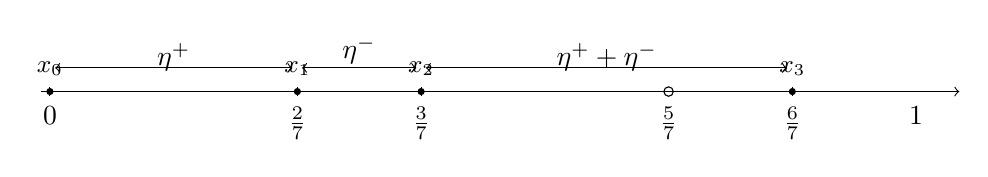
\begin{tikzpicture}[x=11cm,y=1cm]
  \draw[->] (-0.01,0) -- (1.05,0);
  \node[below] at (1,-0.07) {$1$};
  \fill (0,0) circle (1.3pt);
    \draw (0,0.06)--(0,-0.06);
    \node[below] at (0,-0.07) {$0$};        \node[above] at (0,0.08) {\small $x_0$};
  \fill (0.285714,0) circle (1.3pt);
    \draw (0.285714,0.06)--(0.285714,-0.06);
    \node[below] at (0.285714,-0.07) {$\tfrac27$};  \node[above] at (0.285714,0.08) {\small $x_1$};
  \fill (0.428571,0) circle (1.3pt);
    \draw (0.428571,0.06)--(0.428571,-0.06);
    \node[below] at (0.428571,-0.07) {$\tfrac37$};  \node[above] at (0.428571,0.08) {\small $x_2$};
  \fill (0.857143,0) circle (1.3pt);
    \draw (0.857143,0.06)--(0.857143,-0.06);
    \node[below] at (0.857143,-0.07) {$\tfrac67$};  \node[above] at (0.857143,0.08) {\small $x_3$};
  \draw (0.714286,0) circle (1.7pt);
    \node[below] at (0.714286,-0.07) {$\tfrac57$};
  \draw[<->] (0.006,0.30)--(0.280,0.30);  \node at (0.143,0.44) {$\etap$};
  \draw[<->] (0.291,0.30)--(0.423,0.30);  \node at (0.357,0.52) {$\etam$};
  \draw[<->] (0.434,0.30)--(0.851,0.30);  \node at (0.643,0.44) {$\etap+\etam$};
\end{tikzpicture}
\caption{The orbit for $a=\tfrac37$, $N=4$ on $[0,1)$: four points (filled), with
gap lengths $\etap=\tfrac27$, $\etam=\tfrac17$, and the corner gap
$\etap+\etam=\tfrac37$ from $x_2$ to $x_3$.  The corner skips the missing midpoint
$v+\etap=\tfrac57$ (open circle), which first appears only at index
$j+\mpl=4=N$, off the end.}
\label{fig:example}
\end{figure}

The gap $x_3-x_2=\tfrac37$ is the corner.  Here $v=x_2=\tfrac37$ has
$j=\code{canMul}\,v=1$ and $v'=x_3=\tfrac67$ has $j'=2$; both index conditions
fail, $j+\mpl=4\ge N$ and $j'+\mmi=4\ge N$.  The discriminant holds,
$j=1<\mmi=2$, and indeed $v'=v+\etap+\etam=\tfrac37+\tfrac27+\tfrac17=\tfrac67$,
realized at index $j+\mpl-\mmi=2$.  The missing midpoint is
$v+\etap=\tfrac57$, and $\tfrac57\notin\orb(a,4)$ (Theorem~\ref{thm:L2}): it
first appears at index $j+\mpl=4=N$, off the end.  The period argument is
visible numerically---the minimal period here is $q=7$, while $\mpl+\mmi=5$, so
there is no period $d$ at all in the window $(\mpl,\mpl+\mmi)=(3,5)$, and the
collision that case~$k<j$ would require cannot occur.

% =====================================================================
\section{The Lean 4 Formalization}\label{sec:lean}
% =====================================================================

The formalization is a single self-contained module,
\code{ThreeGap.lean}, of about $1{,}480$ lines, depending only on
Mathlib.  It is available in the public repository~\cite{KunertThreeGap2026}.  This section
records its architecture, the design decisions behind it, the correspondence
with the mathematics above, and what a reader must trust.

\subsection{Architecture}

The module follows the order of Sections~\ref{sec:setup}--\ref{sec:corner}.  A
first block builds the orbit, the sorted enumeration, the gap multiset and
\code{gaps\_sum\_eq\_one}, and the distinct-count reduction
\code{three\_gap\_card\_le\_three\_of\_subset}.  A second block introduces the
positive points, the two returns $\etap,\etam$, and their minimality.  A third
recovers the index structure (\code{mulFiber}, \code{canMul}, $\mpl$, $\mmi$) and
proves the fractional-part shift identities.  Cases A and B occupy the
forward and backward ``index-bridge'' blocks, ending in \code{gap\_eq\_etaPos}
and \code{gap\_eq\_etaNeg}.  The final block is the corner: the discriminant
\code{corner\_canMul\_lt\_mMinus}, the $M$-circle infrastructure
(\code{orbit\_mono}, \code{etaPos\_eq\_extend}, \code{etaNeg\_eq\_extend}), the
empty-gap lemmas \code{corner\_noPoint\_lo} and \code{corner\_noPoint\_hi}, the
midpoint argument inside \code{corner\_gap}, and finally
\code{neighbour\_gap\_in\_returns}, \code{gaps\_subset\_returns}, and
\code{three\_gap\_card\_le\_three}.

\subsection{Design decisions}

\begin{itemize}
\item \emph{$[0,1)$ via \code{Int.fract}, not \code{AddCircle}.}  Keeping points
as honest reals in $[0,1)$ lets every difference, order comparison, and interval
membership be a statement about real numbers, handled by \code{linarith},
\code{Int.fract\_eq\_self}, and friends, without transporting across a quotient.
\item \emph{Uniform in $a$.}  The entire development is stated for an arbitrary
$a:\R$; rationality is never assumed and never needed.  The corner step that
would otherwise require it (Theorem~\ref{thm:L2}, Remark~\ref{rmk:uniform}) is
absorbed by the period argument.  This is the single most important difference
from the van Ravenstein--Mayero route.
\item \emph{\code{noncomputable}.}  Order and equality on $\R$ are noncomputable
in Lean, so \code{orbit}, \code{sortedVal}, \code{canMul}, the returns, etc.\ are
all \code{noncomputable}.  This is irrelevant to proving and keeps definitions
faithful to the mathematics.
\end{itemize}

\subsection{Correspondence with the paper}

Table~\ref{tab:correspondence} pairs the principal objects and results above with
their Lean names and line numbers in \code{ThreeGap.lean}.

\begin{table}[ht]
\centering
\begin{tabular}{lll}
\hline
Paper & Lean declaration & line\\
\hline
Orbit $\orb(a,N)$, count $k$        & \code{orbit}, \code{orbitCard}            & 54, 73\\
Sorted points $x_i$                 & \code{sortedVal}                          & 85\\
Gap multiset; $\code{gapAt}$        & \code{gaps}, \code{gapAt}                 & 96, 158\\
Gaps sum to $1$ (Lem.~\ref{lem:sum-one}) & \code{gaps\_sum\_eq\_one}            & 106\\
Reduction (Lem.~\ref{lem:reduction})& \code{three\_gap\_card\_le\_three\_of\_subset} & 190\\
Returns $\etap,\etam$ (Def.~\ref{def:returns}) & \code{etaPos}, \code{etaNeg}   & 247, 252\\
Return minimality (Lem.~\ref{lem:return-min}) & \code{no\_orbit\_below\_etaPos}, & 274,\\
                                    & \quad\code{le\_one\_sub\_etaNeg}          & 292\\
Canonical index                     & \code{canMul}                             & 475\\
Return indices $\mpl,\mmi$          & \code{mPlus}, \code{mMinus}               & 579, 771\\
Shift identity (Lem.~\ref{lem:shift})& \code{fract\_index\_shift}               & 651\\
No point between (Lem.~\ref{lem:npb})& \code{noPointBetween}, \code{noPointBetween\_neg} & 698, 811\\
Case A (Prop.~\ref{prop:caseA})     & \code{gap\_eq\_etaPos}                     & 736\\
Case B (Prop.~\ref{prop:caseB})     & \code{gap\_eq\_etaNeg}                     & 853\\
Discriminant (Lem.~\ref{lem:hP1})   & \code{corner\_canMul\_lt\_mMinus}         & 1104\\
Returns preserved (Lem.~\ref{lem:returns-preserved}) & \code{etaPos\_eq\_extend}, & 1059,\\
                                    & \quad\code{etaNeg\_eq\_extend}            & 1076\\
L1, L3 (Lem.~\ref{lem:L1L3})        & \code{corner\_noPoint\_lo}, \code{corner\_noPoint\_hi} & 1175, 1225\\
Corner gap; L2 (Prop.~\ref{prop:corner}, Thm.~\ref{thm:L2}) & \code{corner\_gap} & 1272\\
Classification                      & \code{neighbour\_gap\_in\_returns}        & 1428\\
Main theorem (Thm.~\ref{thm:main})  & \code{three\_gap\_card\_le\_three}        & 1461\\
Sum relation (\S\ref{subsec:example} text) & \code{three\_gap\_lengths\_eq}     & 1475\\
\hline
\end{tabular}
\caption{Correspondence between the paper and \code{ThreeGap.lean}.}
\label{tab:correspondence}
\end{table}

\subsection{Scope of trust}

What must one trust to accept Theorem~\ref{thm:main}?  Running
\code{\#print axioms three\_gap\_card\_le\_three} reports
\[
  \code{[propext, Classical.choice, Quot.sound]} ,
\]
the three axioms on which Mathlib itself is built.  Nothing specific to this
development is postulated: there is no \code{sorry} and no project-local
\code{axiom}.  Beyond these three axioms, the trusted base is the Lean~4 kernel
that checks the proof term and the small amount of Mathlib API the module
invokes (finite sets, \code{Int.fract}, order embeddings of finite sets,
\code{linarith}/\code{omega} producing checkable certificates).  In particular,
correctness does not depend on the informal exposition of this paper: a reader
who distrusts the prose can recompile the module and inspect the axiom list.

% =====================================================================
\section{Related Work}\label{sec:related}
% =====================================================================

The three-gap theorem has many proofs, and being explicit about the proof
landscape is essential for stating our contribution honestly.

\emph{Classical proofs.}  Steinhaus's conjecture was first proved in the late
$1950$s by S\'os~\cite{Sos1958}, Sur\'anyi~\cite{Suranyi1958}, and
\'Swierczkowski~\cite{Swierczkowski1959}, by elementary number-theoretic and
combinatorial means.  Liang~\cite{Liang1979} later gave a famously short
``rigid gap'' proof.  We stress that Liang's argument is already \emph{uniform}:
it applies verbatim to every rotation number, rational or irrational, with no
case split.  Thus uniformity is not by itself a new feature of any proof, and we
make no such claim; we claim only a uniform \emph{formalization} via the
first-return route.

\emph{The first-return route.}  Slater~\cite{Slater1967} studied the gaps and
steps of $n\theta\bmod1$ directly, and van Ravenstein~\cite{vanRavenstein1988}
organized the proof around the two return times and the continued-fraction
expansion of $\theta$, assuming $\theta$ irrational.  Our formalization follows
this route, and the corner argument of Section~\ref{sec:corner} is exactly the
step at which we depart from it: where van Ravenstein invokes irrationality to
exclude index collisions, we exclude them by the period/minimality bound, which
holds for all~$a$.

\emph{Dynamical and geometric proofs.}  Marklof and
Str\"ombergsson~\cite{MarklofStrombergsson2017} derive the theorem from the
geometry of the space of unimodular lattices, a viewpoint that also yields
higher-dimensional generalizations.  Recent expositions give short geometric
proofs through Farey fractions and lattice configurations~\cite{Geometric2023}.
Berth\'e and Reutenauer~\cite{BertheReutenauer2024} survey the result and its
links to Sturmian words and continued fractions.

\emph{Formalization.}  The only prior formal proof we are aware of is
Mayero's~\cite{Mayero2000}, carried out in Coq (now Rocq) and following van
Ravenstein; like its model it is restricted to irrational rotation numbers.  At
the time of writing the theorem is absent from Mathlib, and we know of no Lean
or Isabelle formalization.  Our development is therefore, to our knowledge, the
first in Lean~4 and the first machine-checked proof---in any system---valid
uniformly for rational and irrational~$a$.  Its place in the landscape is
narrow and concrete: a machine-checked rendering of the first-return proof,
made uniform.

% =====================================================================
\section{Discussion}\label{sec:discussion}
% =====================================================================

\emph{Towards Mathlib.}  Because the three-gap theorem is a named classical
result still missing from Mathlib, a natural next step is to distil the module
into a library contribution.  Two adaptations would help: phrasing the statement
over \code{AddCircle} (the library's preferred model of $\R/\Z$) in addition to
the \code{Int.fract} form used here, and isolating the handful of general-purpose
lemmas about \code{Int.fract} and sorted finite sets that the proof uses.

\emph{Relation to the companion work.}  The orbit $\orb(a,N)$ studied here is,
for rational $a=\alpha/\beta$, precisely the projected point set of a
one-dimensional rational cut-and-project construction, whose gap sequence and
its period---under both the multiset and set conventions---are the subject of a
companion paper~\cite{Kunert2025}.  The three-gap theorem bounds the number of
distinct gap \emph{lengths} appearing in a single window; the companion work
quantifies how the gap \emph{sequence} repeats.  The two are complementary
slices of the same elementary geometry, each formalized in its own public
repository (\cite{Kunert2025}, \cite{KunertThreeGap2026}).

\emph{Further directions.}  The dynamical proofs point to higher-dimensional
Steinhaus and Slater problems, where the number of gap lengths is governed by
the geometry of higher-rank lattices; formalizing even the planar lattice-space
proof would be a substantial and worthwhile project.  We record these only as
directions, not as claims.

% =====================================================================
\section*{Acknowledgments}
% =====================================================================

The Lean~4 formalization, the proof strategy it encodes---including the
period/minimality argument that closes the corner case---and a first draft of
this article were produced by Anthropic's Claude (Claude Opus~4.8) through the
Claude~Code agent, under the author's direction and iterative coaching.  The
author set the goal and constraints, steered the development, and reviewed the
output, but did not contribute the formal proofs himself.  The correctness of
the main result rests not on this division of labour but on the Lean~4 kernel:
\code{three\_gap\_card\_le\_three} is checked to contain no \code{sorry} and to
depend only on Mathlib's three foundational axioms (Section~\ref{sec:lean}), and
the complete source is public~\cite{KunertThreeGap2026}, so any reader can reproduce the
verification independently.  The author takes full responsibility for the final
text.

% =====================================================================
\begin{thebibliography}{99}
% =====================================================================

\bibitem{BertheReutenauer2024}
Val\'{e}rie Berth\'{e} and Christophe Reutenauer,
``On the Three-Distance Theorem,''
\emph{The Mathematical Intelligencer}, vol.~46, no.~2, pp.~183--188, 2024.
\textsc{doi}: \href{https://doi.org/10.1007/s00283-023-10316-z}%
{10.1007/s00283-023-10316-z}.

\bibitem{Geometric2023}
Tadahisa Hamada,
``A concise geometric proof of the three distance theorem,''
preprint, 2023.
arXiv:\href{https://arxiv.org/abs/2308.11999}{2308.11999}.

\bibitem{Kunert2025}
Dirk Kunert,
\emph{Repository cut-and-project}, version \texttt{v1.4-arxiv}, 2025.\newline
Available at: \url{https://github.com/dkunert/cut-and-project/tree/v1.4-arxiv}.

\bibitem{KunertThreeGap2026}
Dirk Kunert,
\emph{Repository three-gap-theorem-lean} (Lean~4 formalization of the three-gap
theorem), 2026.\newline
Available at: \url{https://github.com/dkunert/three-gap-theorem-lean}.

\bibitem{Liang1979}
Frank M.\ Liang,
``A short proof of the $3d$ distance theorem,''
\emph{Discrete Mathematics}, vol.~28, no.~3, pp.~325--326, 1979.
\textsc{doi}: \href{https://doi.org/10.1016/0012-365X(79)90140-7}%
{10.1016/0012-365X(79)90140-7}.

\bibitem{Mathlib2020}
The mathlib Community,
``The Lean mathematical library,''
\emph{Proceedings of the 9th ACM SIGPLAN International Conference on
Certified Programs and Proofs (CPP 2020)},
pp.~367--381, 2020.
\textsc{doi}: \href{https://doi.org/10.1145/3372885.3373824}%
{10.1145/3372885.3373824}.

\bibitem{MarklofStrombergsson2017}
Jens Marklof and Andreas Str\"{o}mbergsson,
``The Three Gap Theorem and the Space of Lattices,''
\emph{The American Mathematical Monthly}, vol.~124, no.~8, pp.~741--745,
2017.
\textsc{doi}: \href{https://doi.org/10.4169/amer.math.monthly.124.8.741}%
{10.4169/amer.math.monthly.124.8.741}.

\bibitem{Mayero2000}
Micaela Mayero,
``The three gap theorem (Steinhaus conjecture),''
in \emph{Types for Proofs and Programs (TYPES 1999)},
Lecture Notes in Computer Science, vol.~1956, Springer, 2000, pp.~162--173.
Also available as arXiv:\href{https://arxiv.org/abs/cs/0609124}{cs/0609124}.
\textsc{doi}: \href{https://doi.org/10.1007/3-540-44557-9_10}%
{10.1007/3-540-44557-9\_10}.

\bibitem{Moura2021}
Leonardo de Moura and Sebastian Ullrich,
``The Lean~4 theorem prover and programming language,''
\emph{Proceedings of the 28th International Conference on Automated
Deduction (CADE-28)},
LNAI, vol.~12699, pp.~625--635, Springer, 2021.
\textsc{doi}: \href{https://doi.org/10.1007/978-3-030-79876-5_37}%
{10.1007/978-3-030-79876-5\_37}.

\bibitem{Slater1967}
Noel B.\ Slater,
``Gaps and steps for the sequence $n\theta\bmod 1$,''
\emph{Proceedings of the Cambridge Philosophical Society},
vol.~63, no.~4, pp.~1115--1123, 1967.
\textsc{doi}: \href{https://doi.org/10.1017/S0305004100042195}%
{10.1017/S0305004100042195}.

\bibitem{Sos1958}
Vera T.\ S\'{o}s,
``On the distribution mod 1 of the sequence \(n\alpha\),''
\emph{Annales Universitatis Scientiarum Budapestinensis de Rolando
E\"{o}tv\"{o}s Nominatae, Sectio Mathematica}, vol.~1, pp.~127--134, 1958.

\bibitem{Suranyi1958}
J\'{a}nos Sur\'{a}nyi,
``\"{U}ber die Anordnung der Vielfachen einer reellen Zahl mod 1,''
\emph{Annales Universitatis Scientiarum Budapestinensis de Rolando
E\"{o}tv\"{o}s Nominatae, Sectio Mathematica}, vol.~1, pp.~107--111, 1958.

\bibitem{Swierczkowski1959}
Stanis{\l}aw \'{S}wierczkowski,
``On successive settings of an arc on the circumference of a circle,''
\emph{Fundamenta Mathematicae}, vol.~46, pp.~187--189, 1959.
\textsc{doi}: \href{https://doi.org/10.4064/fm-46-2-187-189}%
{10.4064/fm-46-2-187-189}.

\bibitem{vanRavenstein1988}
Tony van Ravenstein,
``The three gap theorem (Steinhaus conjecture),''
\emph{Journal of the Australian Mathematical Society (Series A)},
vol.~45, no.~3, pp.~360--370, 1988.
\textsc{doi}: \href{https://doi.org/10.1017/S1446788700031062}%
{10.1017/S1446788700031062}.

\end{thebibliography}

\end{document}
